\chapter{ソフトウェアロードバランサにまつわる技術}
\label{related}
本章では既存のソフトウェアロードバランサを論ずる上で必要不可欠な高速データプレーンの技術について論ずる.


% \section{概要}
% \label{related:abstract}

% コンテンツ事業者が運用するIPv6シングルスタックネットワークの重要な役割の一つに,IPv4クライアントに対するサービス提供がある.

% この様な技術に類似したものとして,アクセスネットワーク網ではIPv6シングルスタックネットワーク上でIPv4によるインターネット接続をクライアントエッジに提供する手法がある.IPv4aaS(IPv4 as a Service)と呼称し,様々な手法が検討されている\cite{RFC8585}.

% 一方でコンテンツ事業者が運用するネットワークでのIPv4サービス提供においては次項で示す要件を満たす必要があるため,必ずしもアクセスネットワークでのIPv4aaSと同様の方法が適切であるとは限らない.

\section{高速なソフトウェアロードバランサ}
\label{related:rapidlb}

% \subsection{IPv4サービス提供機構に求められる要件}
% \label{related:abstract:requirements}
% IPv6シングルスタックネットワークにおいて,サービス提供サーバがIPv4サービスを提供するためには,以下のような機能を有する必要がある.

% \subsubsection{IPv4クライアントからのアクセス}
% IPv6クライアントと同様に,IPv4クライアントに対しても透過的にサービスを提供する機構を備える必要がある.
% 一般的なサーバクライアントモデルを想定した場合,インターネット上のIPv4クライアントからサービス提供サーバに能動的に接続するためには,FQDN\footnote{Fully Qualified Domain Name. 完全就職ドメイン名}もしくはIPv4アドレスを指定出来る必要がある.


% \subsubsection{スケーラビリティ}
% 近年のコンテンツ事業者のネットワークでは,サービスのニーズに合わせて柔軟にスケールアウト\footnote{水平スケール.同等性能の機器を増減させることでサービス容量を拡大・縮小可能なモデル.}可能な設計であることが重要視されている\cite{5550998}.同様にIPv4サービスの提供手法に関しても,事業者のIPv4サービス規模の変化にあわせて柔軟に拡大・縮小可能なアーキテクチャが求められる.

% 例えば,第\ref{introduction:background:IPv6-single-stack-network:ipv4-service}項でも述べたように,将来的にIPv4クライアントの占める割合がIPv6クライアントに相対して低下していった場合に,既設のIPv6ネットワークへの影響を最小限にしつつ,IPv4サービス提供機構を縮小可能であることが望ましい.


% \subsubsection{IPv4ネットワークへの非依存性}
% 第\ref{introduction:background:IPv6-single-stack-network}項で述べたように,IPv6シングルスタックネットワークのメリットを最大限に活かすためにはIPv4サービスを提供する場合においてもIPv4ネットワーク及びアドレスに極力依存しないことが望ましい.



% \section{IPv4サービス提供手法の分類}
% \label{related:compare}
% 想定されるIPv4サービス提供機構をその技術的差異や狙いを基に以下の3つの手法に分類した.

% \subsection{L7リバースプロキシ}

% \begin{figure}[h]
%     \begin{center}
%       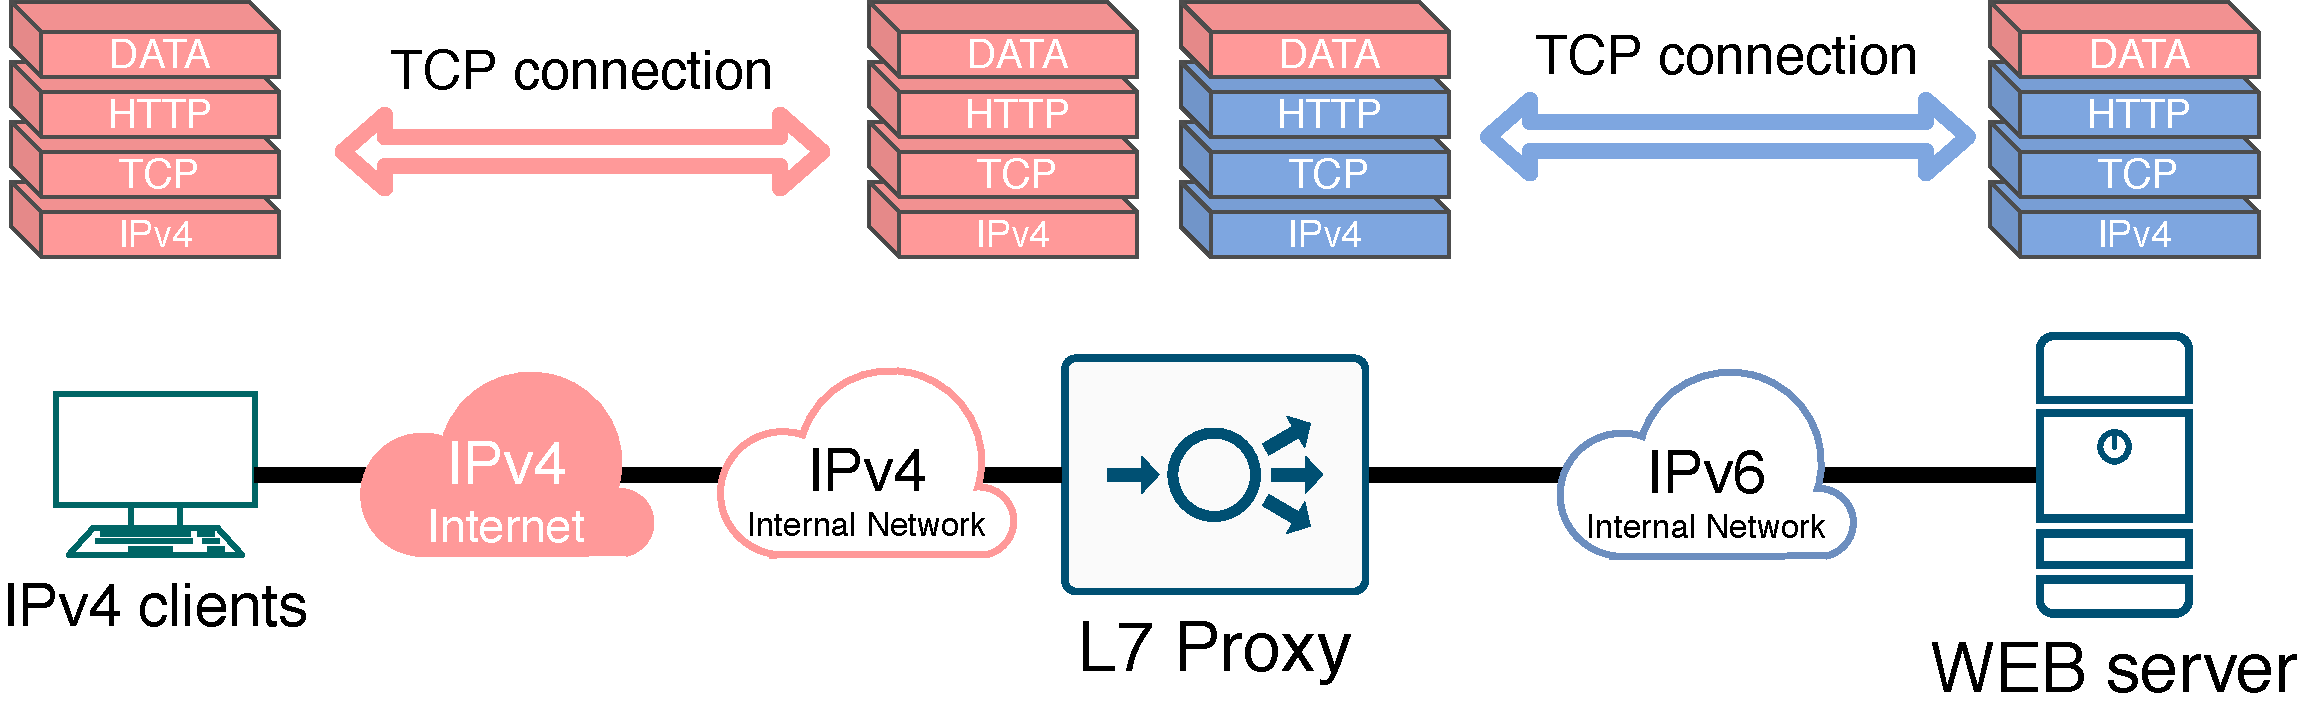
\includegraphics[width=15cm,pagebox=cropbox,clip]{img/L7_proxy_model.pdf}
%     \end{center}
%     \caption{L7リバースプロキシによるIPv4サービス提供}
%     \label{fig:L7_proxy_model}
% \end{figure}


% L7リバースプロキシとは,クライアントからの接続をプロキシサーバがアプリケーション層レベルで終端し,プロキシサーバがクライアントに代わってサーバと接続する機構である\cite{Gilly2011}.図\ref{fig:L7_proxy_model}に本手法の構成を簡便に示す.プロキシサーバを用いる構成は,主にWEBサーバへのHTTP接続を負荷分散するための手法として広く採用されている.

% IPv6シングルスタックネットワークにおいてIPv4サービスを提供するためには,IPv4インターネットとの接続点からプロキシサーバまでの間にIPv4ネットワークを配備する必要がある.

% IPv4・IPv6間のプロトコル仕様の差を考慮する必要が無いため互換性に留意する必要が無い点や,MTU\footnote{ここでは一つのパケットに収容可能なデータ量を指す.}を減らさずにアプリケーショントラフィックを伝送可能である点が利点として挙げられる.

% 一方でアプリケーションレイヤーでのコネクション終端やそのステート管理を行う必要があるため,プロキシサーバに負荷が掛かるため高性能な機器の導入が必要になる.

% またスケールアウトを可能にするためにL4LB(Layer4 Load Balancer)\footnote{トランスポート層レベルでの負荷分散を行う機器.}と組み合わせたマルチステージのアーキテクチャを利用する手法が近年主流であるが\cite{Facebook_LB, Google_LB},この手法を採用するためには,L4LB及びプロキシサーバにまでIPv4ネットワークを配備する必要があり,\ref{related:abstract:requirements}項で述べた要件に合致せず,IPv6シングルスタックネットワークのメリットを損なうことになる.



% \subsection{IPv4/IPv6トンネリング}
% \begin{figure}[h]
%     \begin{center}
%       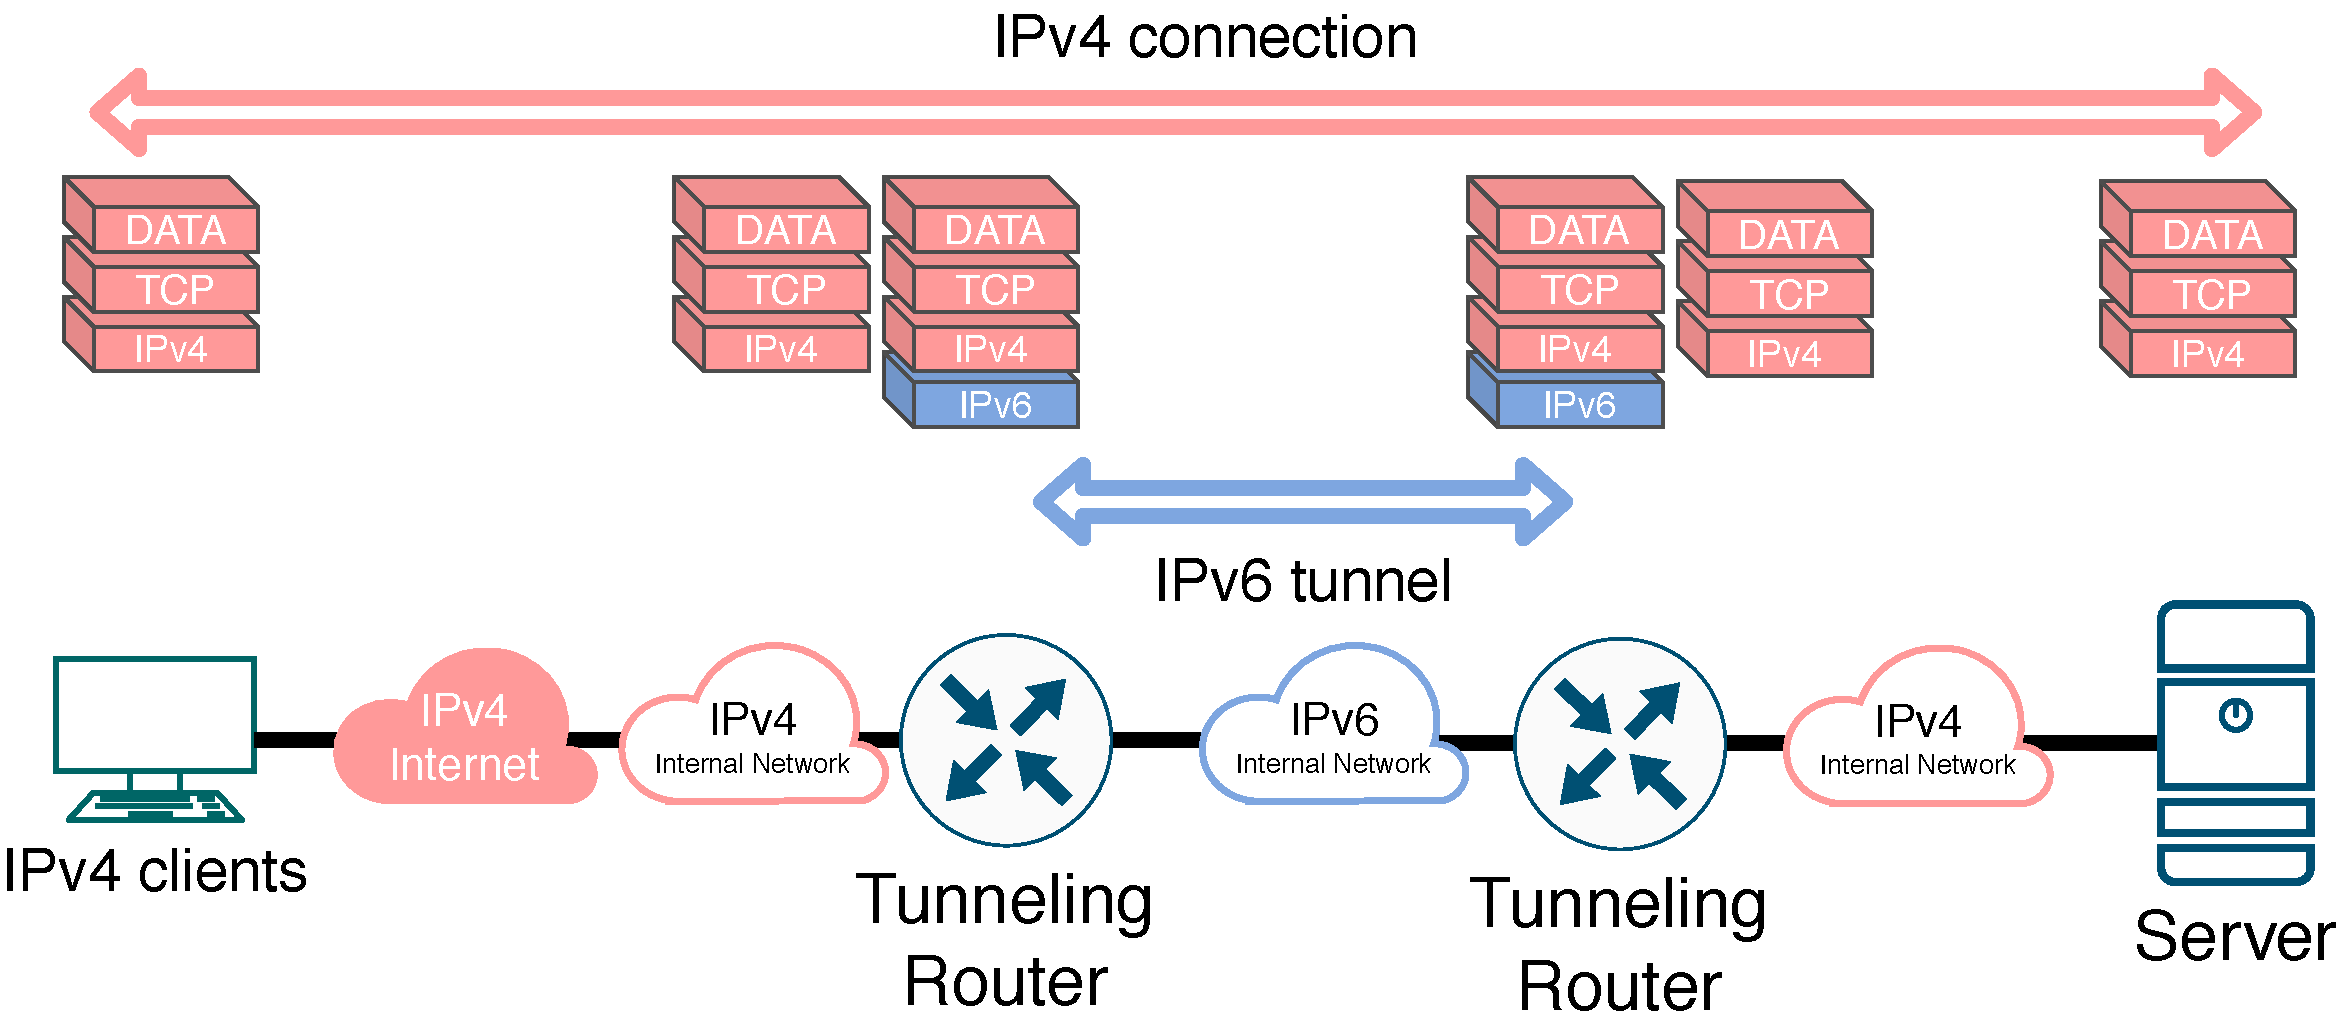
\includegraphics[width=15cm,pagebox=cropbox,clip]{img/Tunneling_model.pdf}
%     \end{center}
%     \caption{IPv4/IPv6トンネリングによるIPv4サービス提供}
%     \label{fig:tunneling_model}
% \end{figure}

% IPv4/IPv6トンネリングとは,IPv4パケットをIPv6パケットによってカプセリングすることでIPv6ネットワークを通過させる手法である.IPv4トラフィックを透過的に利用することが出来るため,アクセスネットワークでのIPv4aaS実現手法として広く利用されている\cite{RFC8585}.図\ref{fig:tunneling_model}に本提供手法の構成を簡便に示す.

% IPv6シングルスタックにおけるIPv4サービス提供手法としては,IPv4クライアントから到達したパケットをトンネルルータによって一度IPv6パケットでカプセリングし,IDC内のIPv6シングルスタックネットワークを通過させ,IPv4サービス提供サーバ上もしくはその直前で再びでカプセリングを解くことで,IPv4提供サーバまでネイティブなIPv4トラフィックを通過させる運用が考えらえる.
% IPv4パケットをそのままサーバまで届けることが出来るため,多種多様なアプリケーションでのサービス提供が可能である.

% しかしながら,トンネルルータとIPv4サービスサーバ間にIPv4ネットワークを配備しなければならず,ToR(Top of rack switch)\footnote{ここではサーバのL2終端を行うイーサネットスイッチを指す.}及びサーバではIPv4/IPV6デュアルスタック運用が必要になるため,第\ref{related:abstract:requirements}項で上げた要件である「IPv4ネットワークへの非依存性」を満たすことが出来ない.また,トンネルプロトコルの多く\cite{6799698}は基本的に1:1もしくは1:Nの接続が基本となるため,スケールアウトさせることが困難である.



% \subsection{IPv4/IPv6トランスレーション}
% \label{related:compare:translation}
% \begin{figure}[h]
%     \begin{center}
%       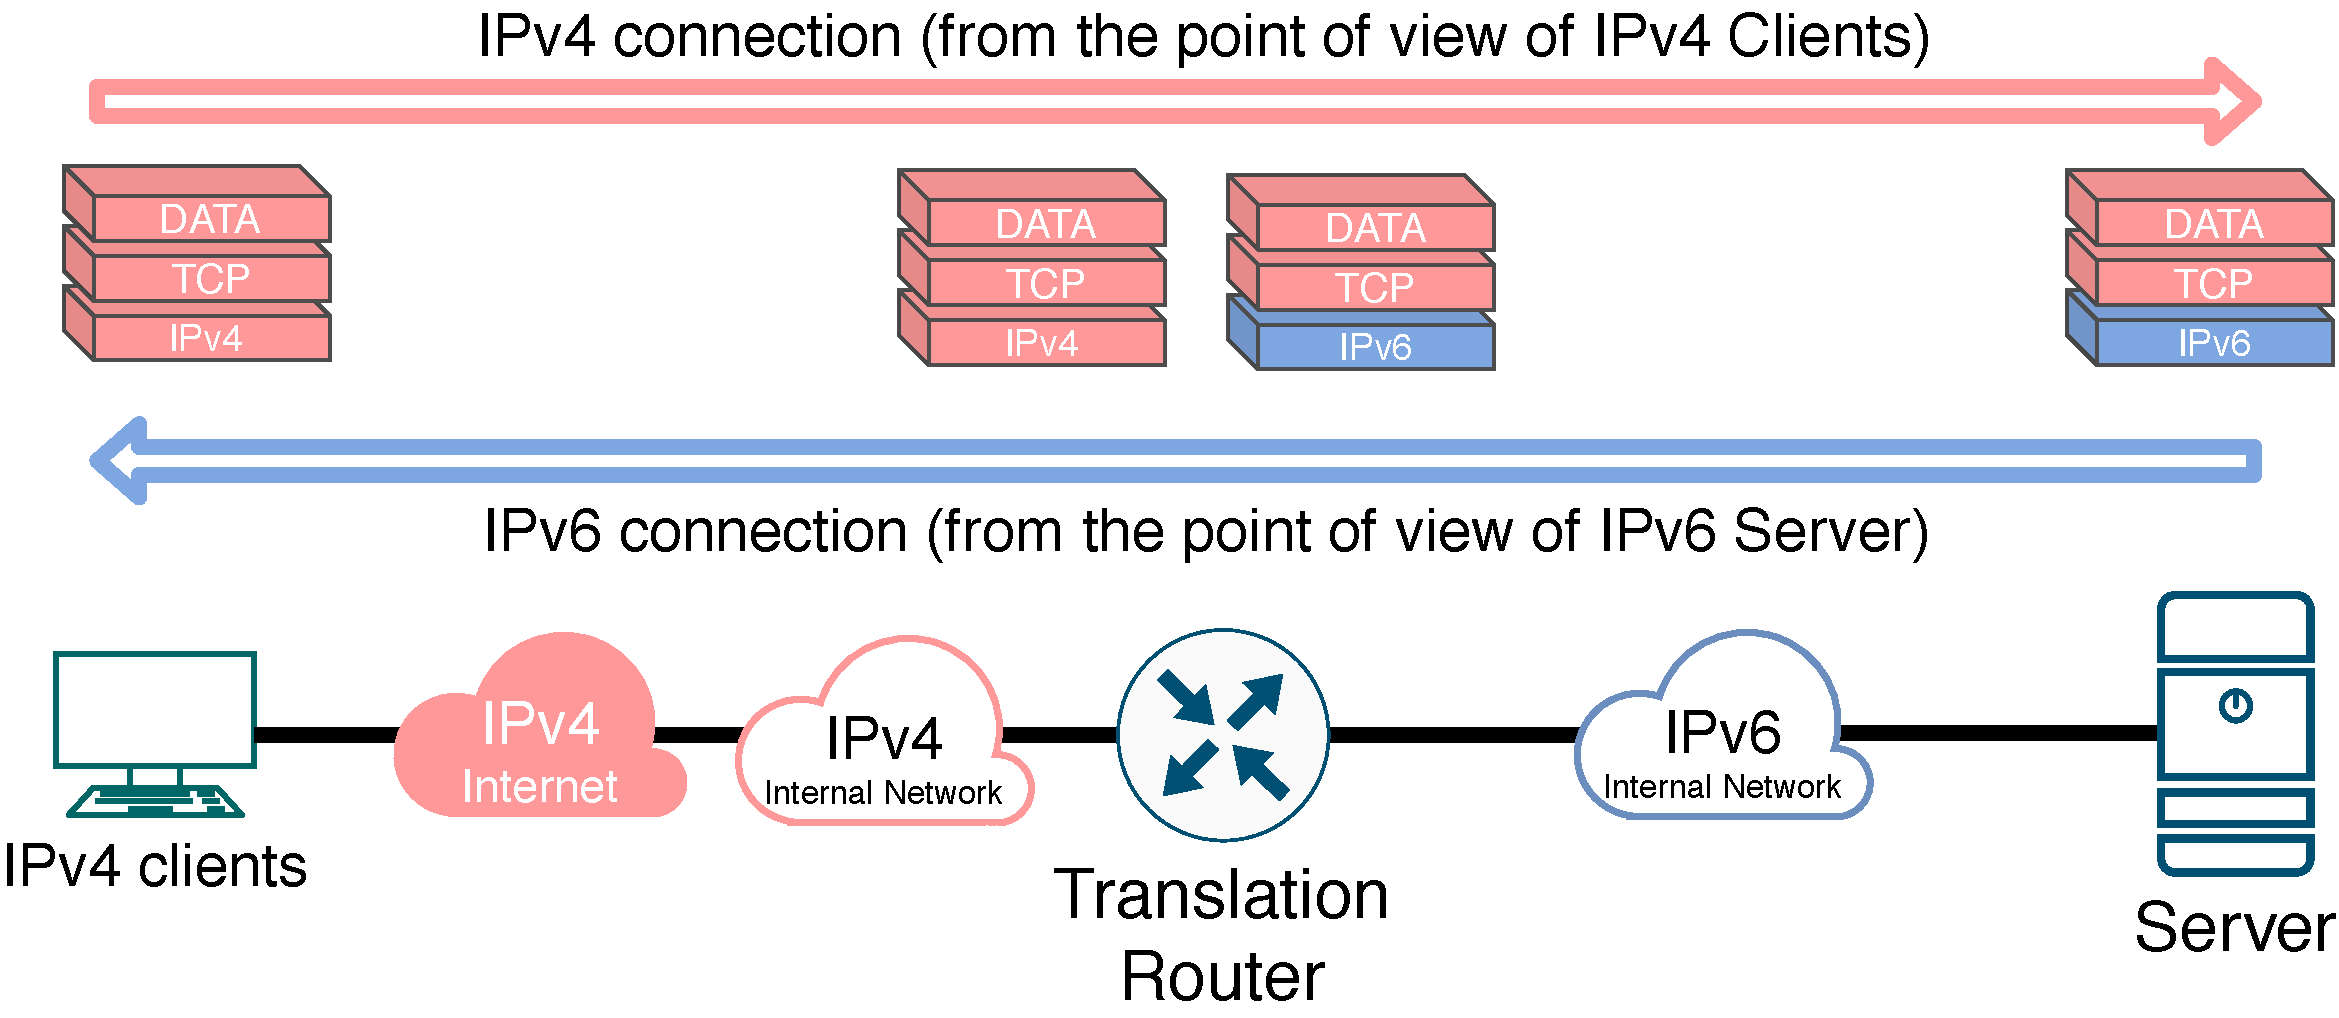
\includegraphics[width=15cm,pagebox=cropbox,clip]{img/translation_model.pdf}
%     \end{center}
%     \caption{IPv4/IPv6トランスレーションによるIPv4サービス提供}
%     \label{fig:tunneling_model}
% \end{figure}

% IPv4/IPv6トランスレーションとは,IPv4パケットとIPv6パケットをIP/ICMP変換アルゴリズムを利用して相互に変換する手法である.$1:N$の関係でアドレス・ポート変換を行うステートフルなNAT64\cite{RFC6146}と,$1:1$でアドレス変換を行うステートレスなSIIT\cite{RFC7915}が定義されている.IPv4ネットワークとIPv6ネットワークの境界に位置する変換ルータにより,相互にプロトコル変換が行われる.

% IPv4/IPv6トランスレーションではIPv4アドレスをIPv6アドレスとして表現することが要求されるが,変換プレフィックスと呼ばれるIPv6ネットワークプレフィックスにIPv4アドレスを埋め込むことで,任意のIPv4アドレスをIPv6ホストから認識可能な形で表現する.変換プレフィックスにはRFC6052で定義された64:ff9b::/96の他に,運用者が専有可能なGUA(Global Unicast Address)の/96のIPv6プレフィックスを利用することが想定されている\cite{RFC6052}.

% 図\ref{fig:tunneling_model}で示すように,変換ルータ以外のホストがIPv4ネットワークに属する必要が無いため,第\ref{related:abstract:requirements}項で述べた「IPv4ネットワークへの非依存性」の面で,他の2手法より優れていると言える.また,IPv4サービスを行うサーバから変換ルータの間はネイティブなIPv6ネットワークで接続可能なため,ECMP(Equal Cost Multi Path)\cite{rfc2992}による経路の冗長化が可能なほか,ステートレスモードでは変換ルータのスケールアウトが可能な点で,IPv6シングルスタックネットワークにおけるIPv4サービス提供に求められる要件を満たしやすい.

% またサーバ側においても,アクセスコントロールの設定やログデータの管理など,IPv4とIPv6で別個に行われていた制御の削減が期待される.サーバ・アプリケーション管理者はネットワークプロトコルを意識したオペレーションをする必要がなく,運用効率改善の点でメリットが非常に大きい.

% 一方でIPv4とIPv6のプロトコル実装に差があるため,コンテンツ事業者のサービスの内容によってはサービス影響を考慮する必要がある点は留意すべきである.


% \section{本章のまとめ}
% \ref{related:abstract:requirements}項で述べた評価要件を尺度として,各IPv4サービス提供手法の特徴を比較した.これを表\ref{table:related_compare}に示す.

% 基本的なIPv4サービス提供手法の必要要件であるIPv4クライアントからのアクセスは各手法とも充足可能な一方,スケーラビリティの面では1:1/1:Mの接続が必須になるIPv4/IPv6トンネリング手法が他の手法から大きく劣る.
% またL7リバースプロキシ手法はスケールアウト可能なアーキテクチャであるが,L4LB及びプロキシサーバLまでIPv4ネットワークを配備する必要があるため,IPv4ネットワークへの依存性が大きい.

% IPv4/IPv6トランスレーション手法はスケールアウトが可能であり,IPv4ネットワークへの依存性が小さいため,IPv6シングルスタックネットワーク環境でのIPv4サービス提供手法として最も要件に適合する.


% \begin{table}[h]
%   \label{table:related_compare}
%   \caption{IPv4サービス提供手法の比較}
%   \centering
%   \resizebox{\textwidth}{!}{%
%   \begin{tabular}{lccc}
%   \hline
%   \multicolumn{1}{c}{手法名} & IPv4クライアントからのアクセス & \multicolumn{1}{l}{スケーラビリティ} & \multicolumn{1}{l}{IPv4ネットワークへの依存性} \\ \hline
%   (参考)IPv4/IPv6デュアルスタック & 可能 & 困難 & 大 \\
%   L7 リバースプロキシ & 可能 & スケールアウト可 & 中 \\
%   IPv4/IPv6 トンネリング & 可能 & 困難 & 中 \\
%   IPv4/IPv6 トランスレーション & 可能 & スケールアウト可 & 小 \\ \hline
%   \end{tabular}%
%   }
% \end{table}
%%% Local Variables:
%%% mode: japanese-latex
%%% TeX-master: "../thesis"
%%% End: